% --------------------------------------------
% Fourier Epicycles - Main Document
% Uses tex-content-publisher template
% --------------------------------------------

% Load external preamble (base template)
\def\tcppath{../../tex-content-publisher/}
\input{\tcppath preamble}

% Load custom local colors (override)
% ============================================
% OVERRIDE LOCAL DE COLORES - Fourier Epicycles
% Tema: Pastel armonioso (estilo IEC-61131-3)
% Ideal para LinkedIn - colores suaves y llamativos
% ============================================

% Fondo pastel claro
\definecolor{ColorBg}{HTML}{F2F6FC}
\pagecolor{ColorBg}

% Header
\definecolor{ColorHeadLeft}{HTML}{F8F3ED}

% Footer
\definecolor{ColorLineFoot}{HTML}{ded6d6}

% Texto principal (teal elegante)
\definecolor{ColorBlueText}{HTML}{0D9488}
\definecolor{customcolor}{HTML}{0D9488}

% Cajas (verde menta pastel)
\definecolor{ColorBoxTitle}{HTML}{CCFBF1}  % Teal muy claro
\definecolor{ColorBox}{HTML}{F0FDFA}       % Teal casi blanco

% Debug (para valores inline - coral suave)
\definecolor{ColorDebugFill}{HTML}{FFEDD5}  % Orange muy claro
\definecolor{ColorDebugFrame}{HTML}{F97316} % Orange

% Código
\definecolor{codegreen}{HTML}{059669}      % Emerald
\definecolor{codegray}{HTML}{64748B}       % Slate
\definecolor{codepurple}{HTML}{7C3AED}     % Violet
\definecolor{backcolour}{HTML}{F8FAFC}     % Slate muy claro
\definecolor{ColorFrame}{HTML}{14B8A6}     % Teal

% Colores adicionales Fourier (pastel pero vibrantes)
\definecolor{primary}{HTML}{14B8A6}        % Teal
\definecolor{secondary}{HTML}{E11D48}      % Rose Strong (mas notorio que anaranjado)
\definecolor{accent}{HTML}{8B5CF6}         % Purple
\definecolor{success}{HTML}{22C55E}        % Green


% Load VS Code-style C++ highlighting from template
\input{\tcppath codestyles/cpp-vscode}

% Additional packages
\usetikzlibrary{arrows.meta, decorations.pathmorphing, calc, positioning}
\usepackage{fontawesome5}

% Hyperref
\hypersetup{
    colorlinks=true,
    linkcolor=ColorBlueText,
    urlcolor=ColorBlueText,
    pdftitle={Fourier Epicycles},
}

% Header/Footer simple
\ihead{
    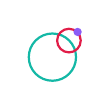
\begin{tikzpicture}[baseline]
        \draw[primary, thick] (0,0) circle (0.3);
        \draw[secondary, thick] (0.21,0.21) circle (0.15);
        \fill[accent] (0.32,0.32) circle (1.5pt);
    \end{tikzpicture}
}
\chead{\textcolor{ColorBlueText}{\bfseries\Large Fourier Epicycles}}
\ohead{\textcolor{primary}{$\sum c_n e^{in\omega t}$}}
\ifoot[\textcolor{codegray}{\small Mathematics + Code}]{\textcolor{codegray}{\small Mathematics + Code}}
\ofoot[\textcolor{codegray}{\small\faGithub\ \href{https://github.com/asdcainicela/fourier-epicycles-cpp}{fourier-epicycles-cpp}}]{\textcolor{codegray}{\small\faGithub\ \href{https://github.com/asdcainicela/fourier-epicycles-cpp}{fourier-epicycles-cpp}}}

% Tables
\arrayrulecolor{primary}

% --------------------------------------------
\begin{document}
    \thispagestyle{plain}
    
\setstretch{1.4}

% Title
\begin{center}
    {\fontsize{44}{52}\bfseries\textcolor{ColorBlueText}{Fourier Epicycles}}
\end{center}

% Content

\begin{minipage}[c]{0.65\textwidth}
    Periodic function:
    \begin{equation}
    f(t) = \sum_{n=-\infty}^{\infty} c_n \cdot e^{i n \omega t}
    \end{equation}
    
    Each term is a rotating vector. The sum generates a chain of epicycles whose endpoint traces $f(t)$.
\end{minipage}
\hfill
\begin{minipage}[c]{0.35\textwidth}
    \begin{tikzpicture}[scale=4]
        \draw[primary!80, thin] (0,0) circle (0.8);
        \draw[-{Stealth[length=2mm]}, primary, line width=1.5pt] (0,0) -- (0.56,0.56);
        \node[primary, font=\small] at (0.15, 0.45) {$|c_1|$};
        \fill[primary] (0,0) circle (0.5pt); % center draw fill
        
        \begin{scope}[shift={(0.56,0.56)}]
            \draw[secondary!80, thin] (0,0) circle (0.4);
            \draw[-{Stealth[length=2mm]}, secondary, line width=1.2pt] (0,0) -- (0.35,0.2);
            \node[secondary, font=\small] at (0.08, 0.28) {$|c_2|$};
            \fill[secondary] (0,0) circle (0.5pt);
            
            \begin{scope}[shift={(0.35,0.2)}]
                \draw[accent!80, thin] (0,0) circle (0.2);
                \draw[-{Stealth[length=1.5mm]}, accent, line width=1pt] (0,0) -- (0.18,0.08);
                \fill[accent] (0,0) circle (0.5pt);
            \end{scope}
        \end{scope}
        
        \draw[curve, thick, dashed, smooth] 
            plot coordinates {
                (1.09, 0.84) (1.12, 0.7) (1.4, 0.5) (1.7, 0.0) 
                (1.9, 0.2) (2.1, 0.9) (1.7, 1.2) 
                (1.4, 1.0) (1.12, 0.9) (1.09, 0.84)
            };
        \fill[curve] (1.09, 0.84) circle (0.5pt);
        \node[secondary, font=\bfseries, anchor=west] at (1.12, 0.84) {$f(t)$};
    \end{tikzpicture}
\end{minipage}

\begin{minipage}[t]{0.47\textwidth}
\vspace{0pt}
\begin{lstlisting}

struct FourierCoefficient {
    int frequency;
    std::complex<double> cn;
    double amplitude;
    double phase;
    // ...
};

\end{lstlisting}
\end{minipage}
\hfill
\begin{minipage}[t]{0.5\textwidth}
\vspace{-5pt}
\begin{tabular}{lcl}
\textbf{Field} & \textbf{Math} & \textbf{Geometry} \\
\hline
frequency & $n$ & Angular velocity \\
cn & $c_n$ & Complex coefficient \\
amplitude & $|c_n|$ & Radius of epicycle \\
phase & $\arg(c_n)$ & Initial angle \\
\end{tabular}
\end{minipage}

\vspace{0.8cm}

% --- DFT ---
\textbf{DFT Computation} (Discrete Fourier Transform)\\
It is the discretization of the Fourier transform that allows computing the Fourier coefficients of a digital signal.
$$
 C_n = \frac{1}{N} \sum_{k=0}^{N-1} z_k \cdot e^{-i \frac{2\pi n k}{N}}
$$

Thus, the coefficient $C_n$ is the value of the transform at frequency $n$, and in code:
\begin{lstlisting}
std::vector<FourierCoefficient> computeDFT(
    const std::vector<std::complex<double>>& points) {
    const size_t N = points.size();
    std::vector<std::complex<double>> spectrum(N);
    kissfft<double> fft(N, false);
    fft.transform(points.data(), spectrum.data());
    
    std::vector<FourierCoefficient> coeffs;
    for (size_t n = 0; n < N; ++n) {
        auto cn = spectrum[n] / double(N);
        coeffs.push_back({(n < N/2) ? (int)n : (int)n-(int)N,
            std::abs(cn), std::arg(cn), cn});
    }
    return coeffs;
}
\end{lstlisting}

\vspace{0.5cm}

Thus, the evaluation of $ \displaystyle f(t) = \sum_n |c_n| \cdot e^{i(n t + \phi_n)}$ in code:
\begin{lstlisting}
std::complex<double> evaluate(
    const std::vector<FourierCoefficient>& coeffs, double t) {
    std::complex<double> z(0, 0);
    for (const auto& c : coeffs)
        z += c.amplitude * std::exp(
            std::complex<double>(0, c.frequency * t + c.phase));
    return z;
}
\end{lstlisting}


\input{animation}
    
\end{document}
